\begin{center}
\vspace*{0.1in}
\begin{Large}
\textbf{PRACTICA DE LABORATORIO N° 01:} \\
\textbf{(Elaboración de Dashboards en Power BI)} \\
\end{Large}
\end{center}
\begin{document}
\section{OBJETIVO:}
\item{
Desarrollar el Informe de Labratorio 01 de Dashboards en Power BI}
\section{REQUERIMIENTOS}
\item{Conocimientos
Para el desarrollo de esta práctica se requerirá de los siguientes conocimientos básicos:\\
- Conocimientos básicos de administración de base de datos Microsoft SQL Server.\\
- Conocimientos básicos de SQL.\\
✓ Software
Asimismo se necesita los siguientes aplicativos:
- Microsoft SQL Server 2016 o superior\\
- Base de datos AdventureWorks2016 o superior\\
- Power BI Desktop.\\
- Tener una cuenta Microsoft registrada en el Portal de Power Bi}\\

\section{CONSIDERACIONES INICIALES}
\item{Generar una carpeta o directorio Power BI en un lugar accesible para guardar los resultados de la práctica.}\\
\\\\\\\\\\\\\\\\\\\\\\\\\\\\
\section{DESARROLLO}

\subsection{RESULTADO Nº01:}
\begin{figure}[httb]
\begin{center}
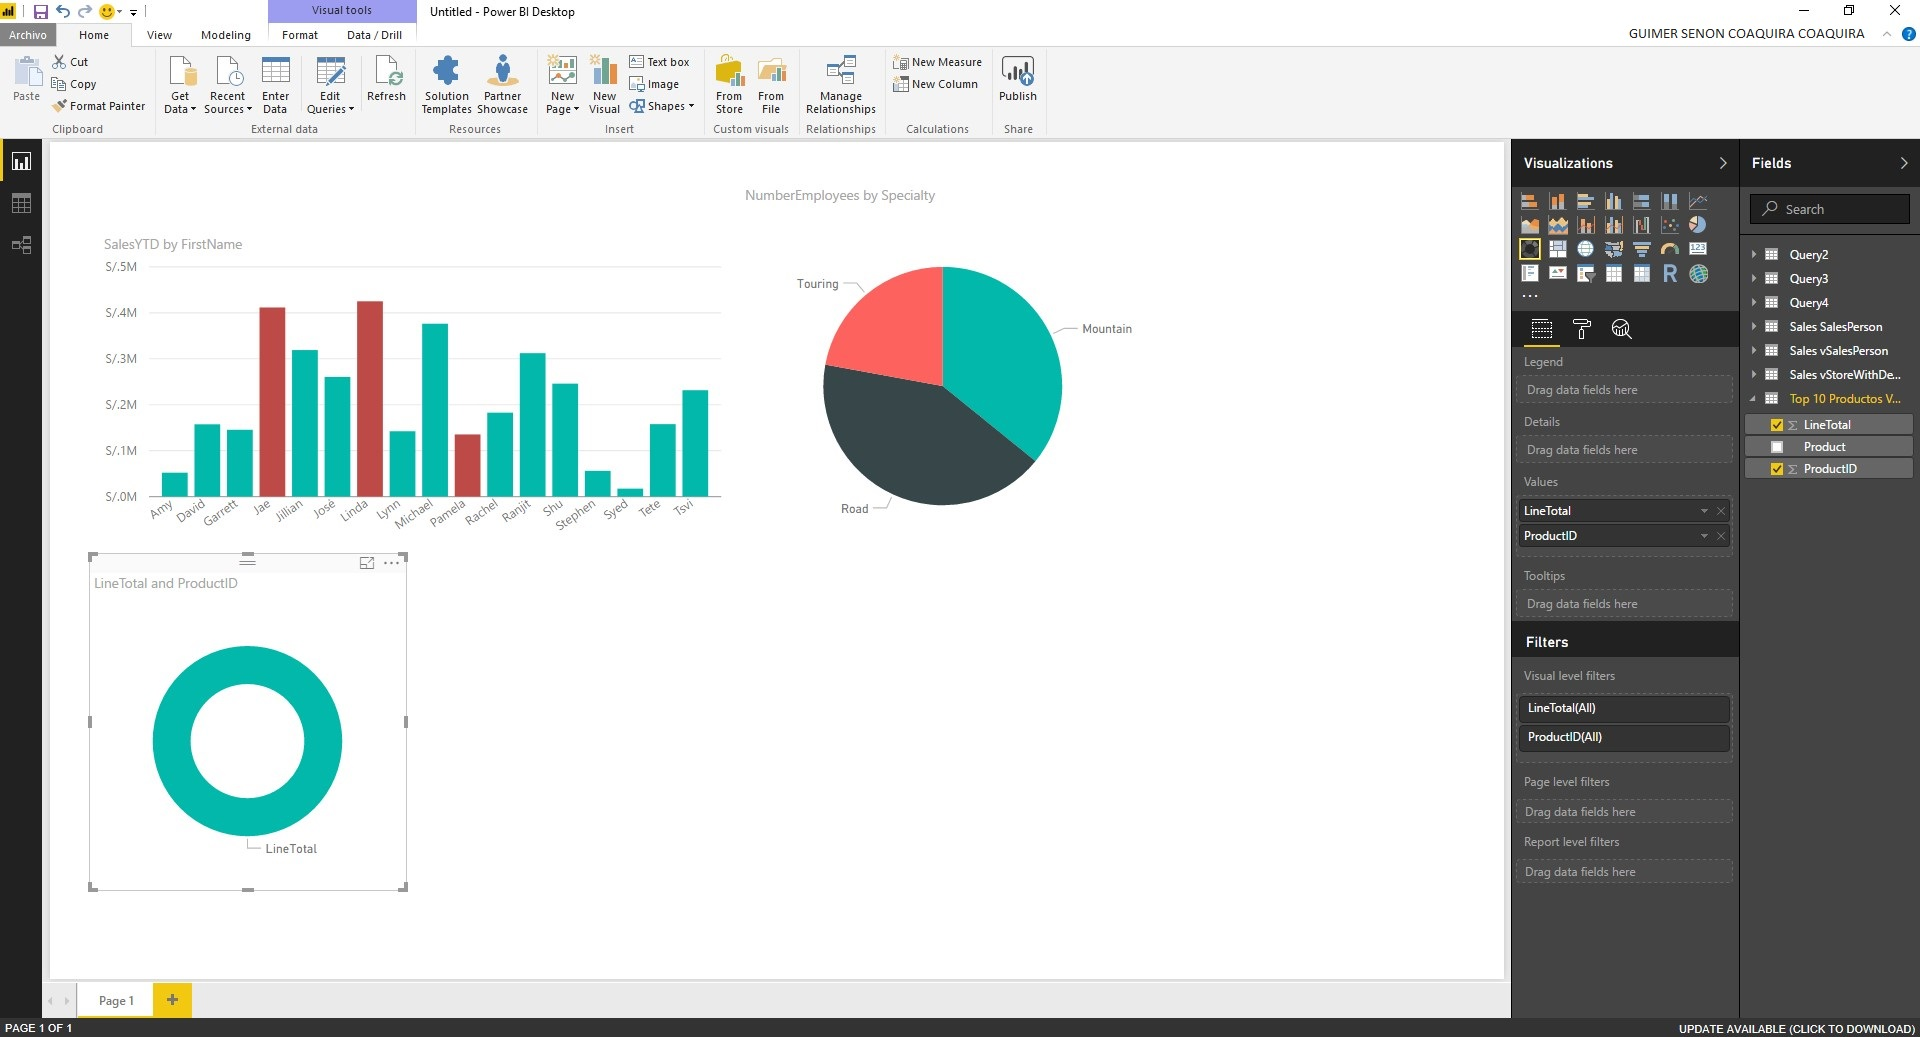
\includegraphics[width=15cm]{./Imagenes/Captura01}
\end{center}
\end{figure}

\subsection{RESULTADO Nº02:}
\begin{figure}[httb]
\begin{center}
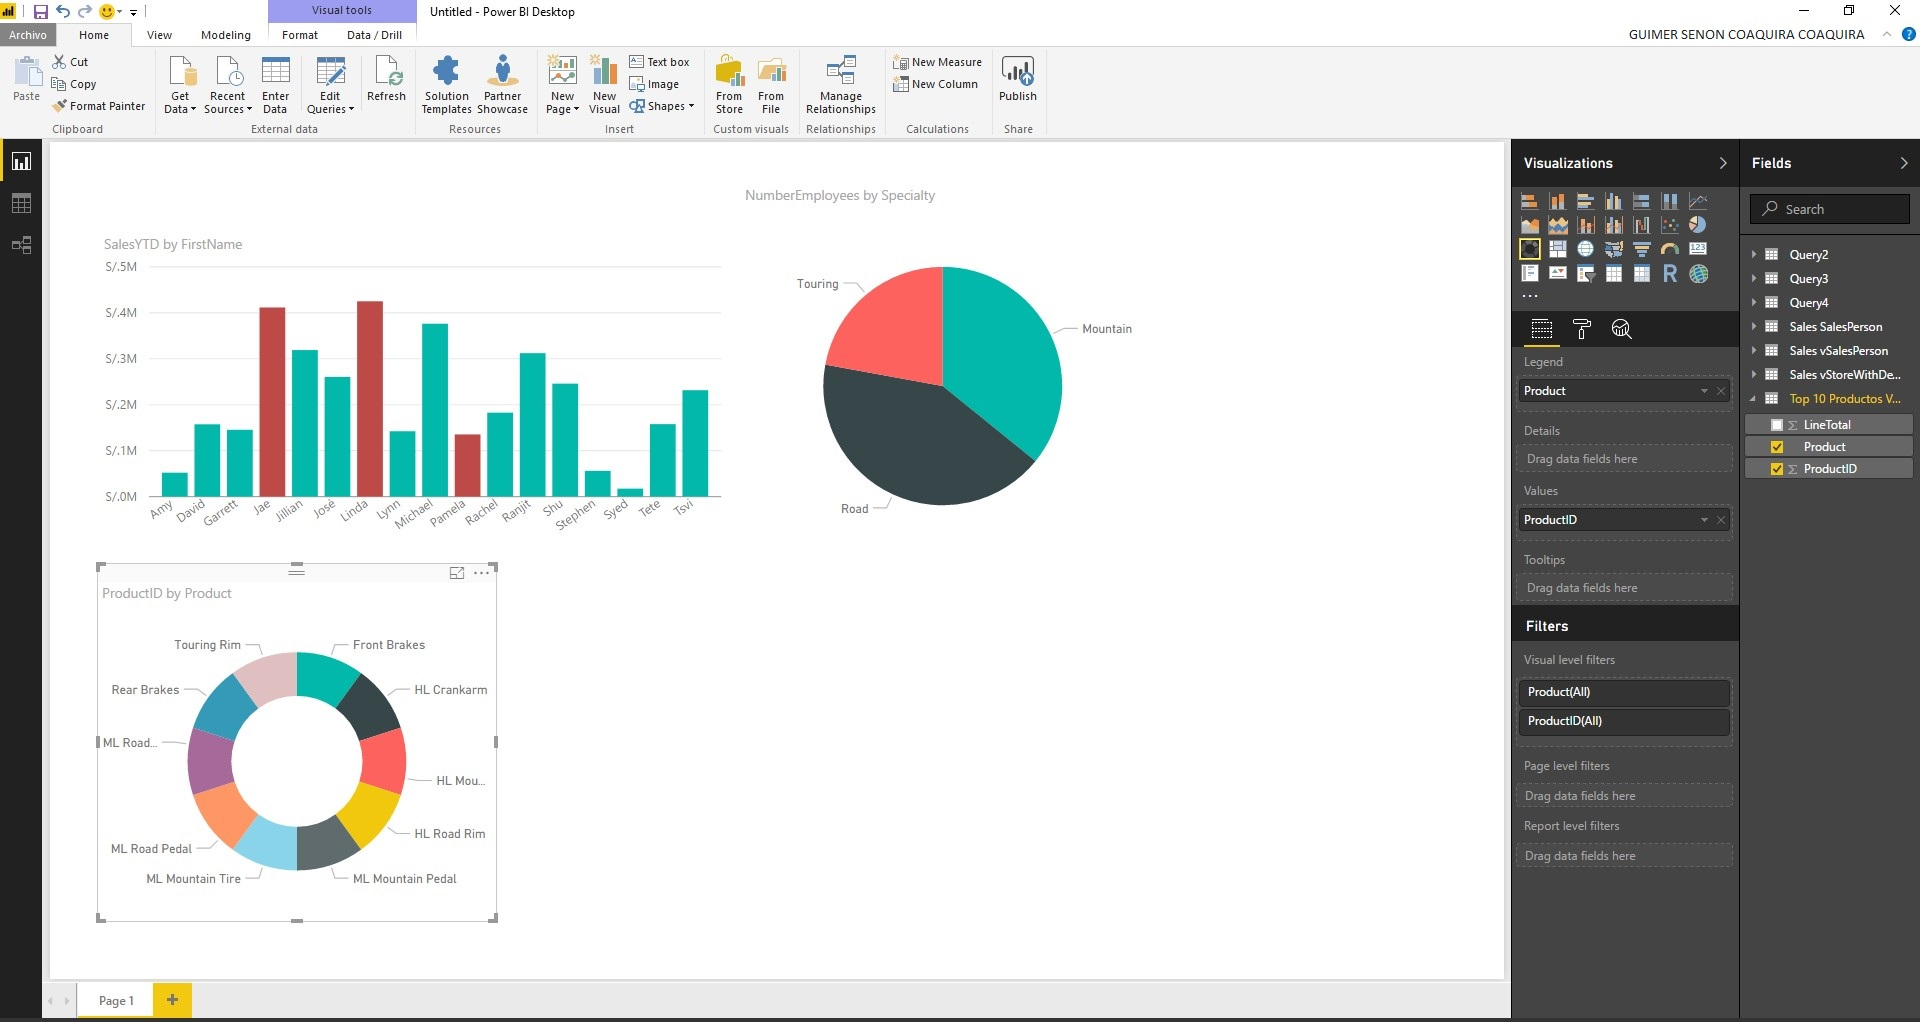
\includegraphics[width=15cm]{./Imagenes/Captura02}
\end{center}
\end{figure}
\newpage
\subsection{RESULTADO Nº03:}
\begin{figure}[httb]
\begin{center}
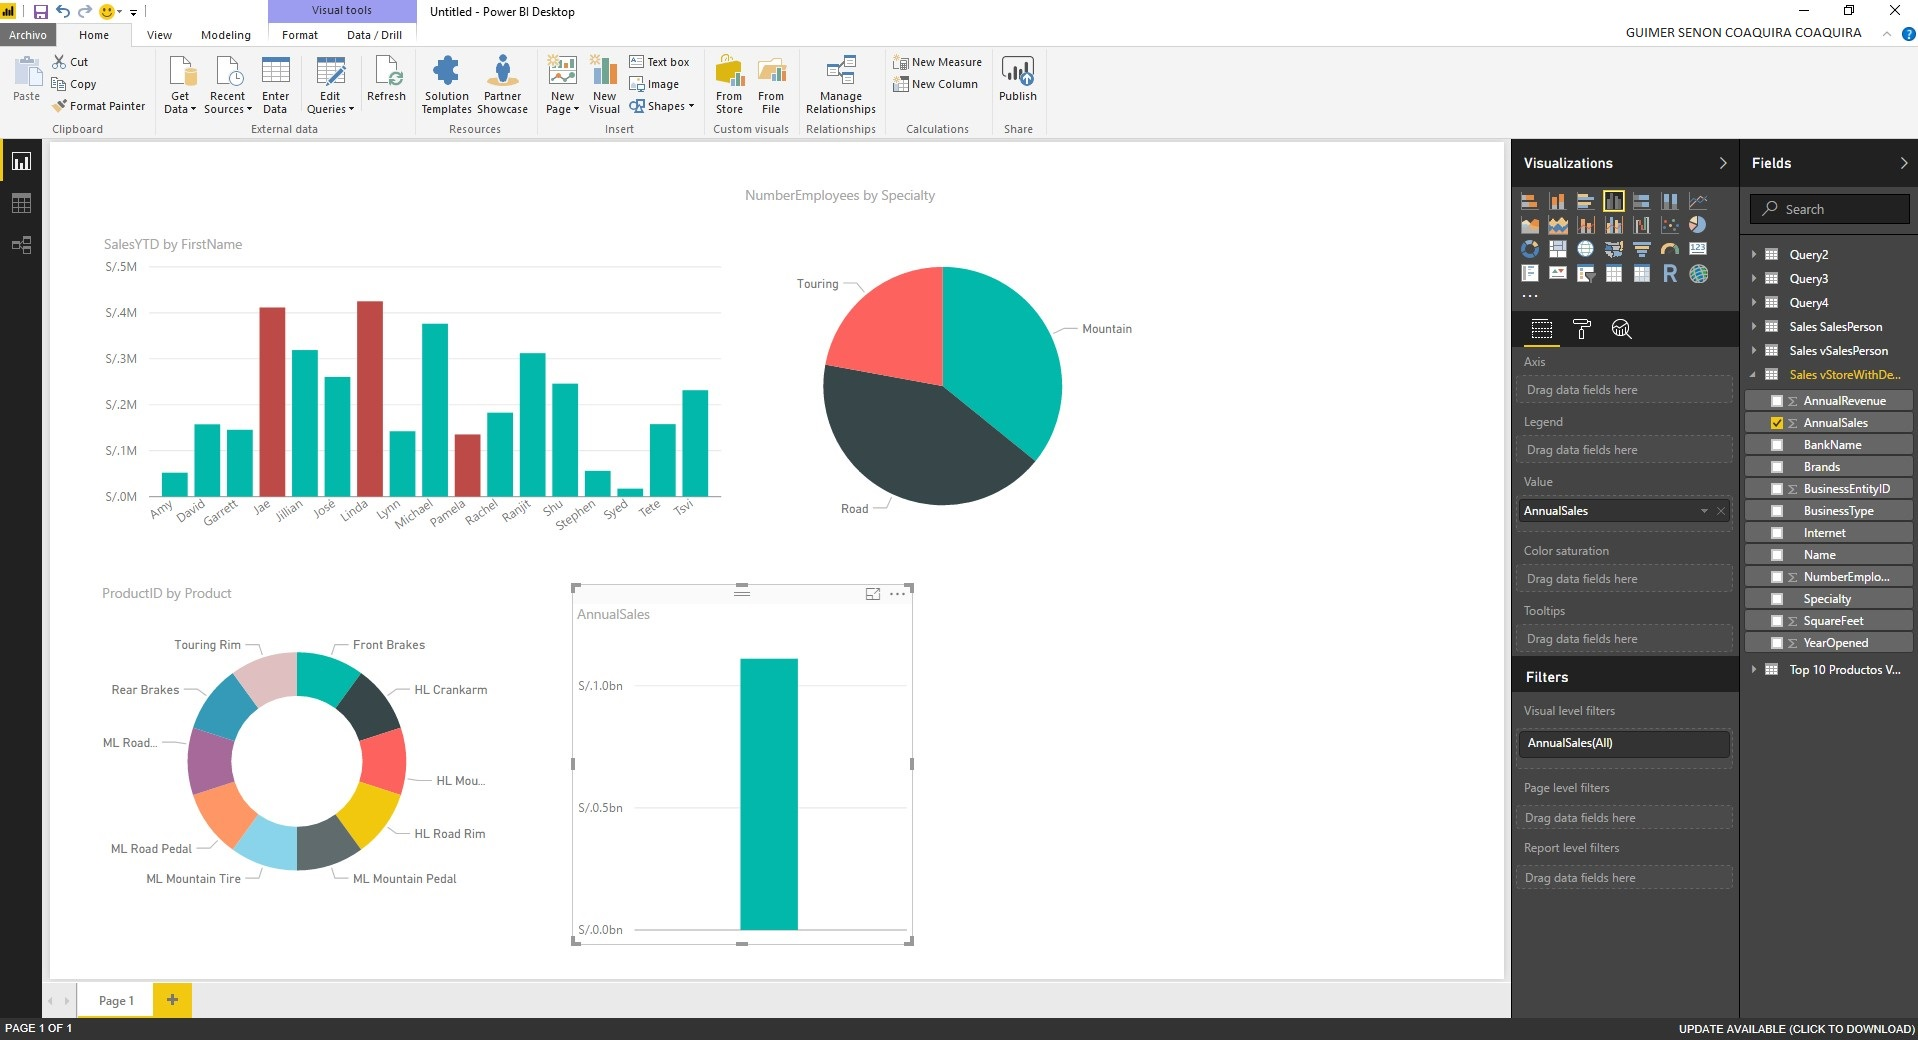
\includegraphics[width=15cm]{./Imagenes/Captura03}
\end{center}
\end{figure}

\subsection{RESULTADO Nº04:}
\begin{figure}[httb]
\begin{center}
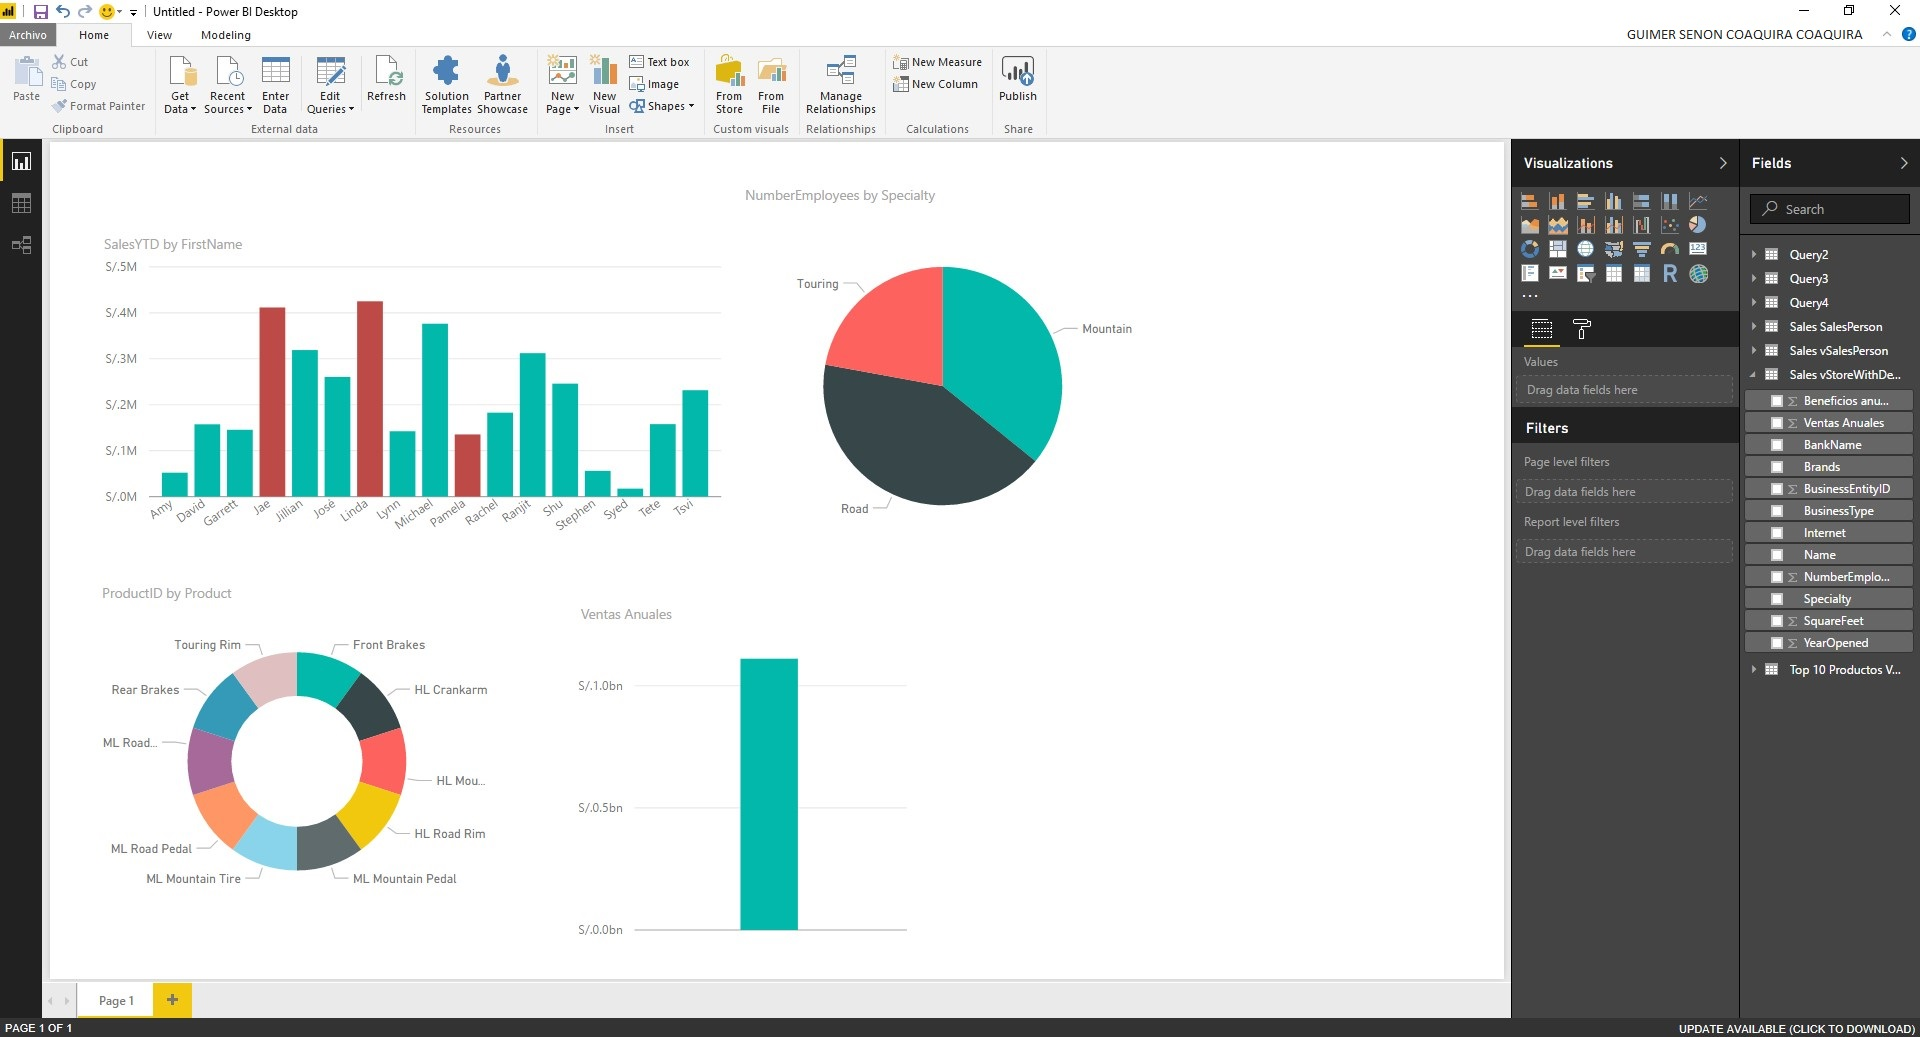
\includegraphics[width=15cm]{./Imagenes/Captura04}
\end{center}
\end{figure}
\newpage
\subsection{RESULTADO Nº05:}
\begin{figure}[httb]
\begin{center}
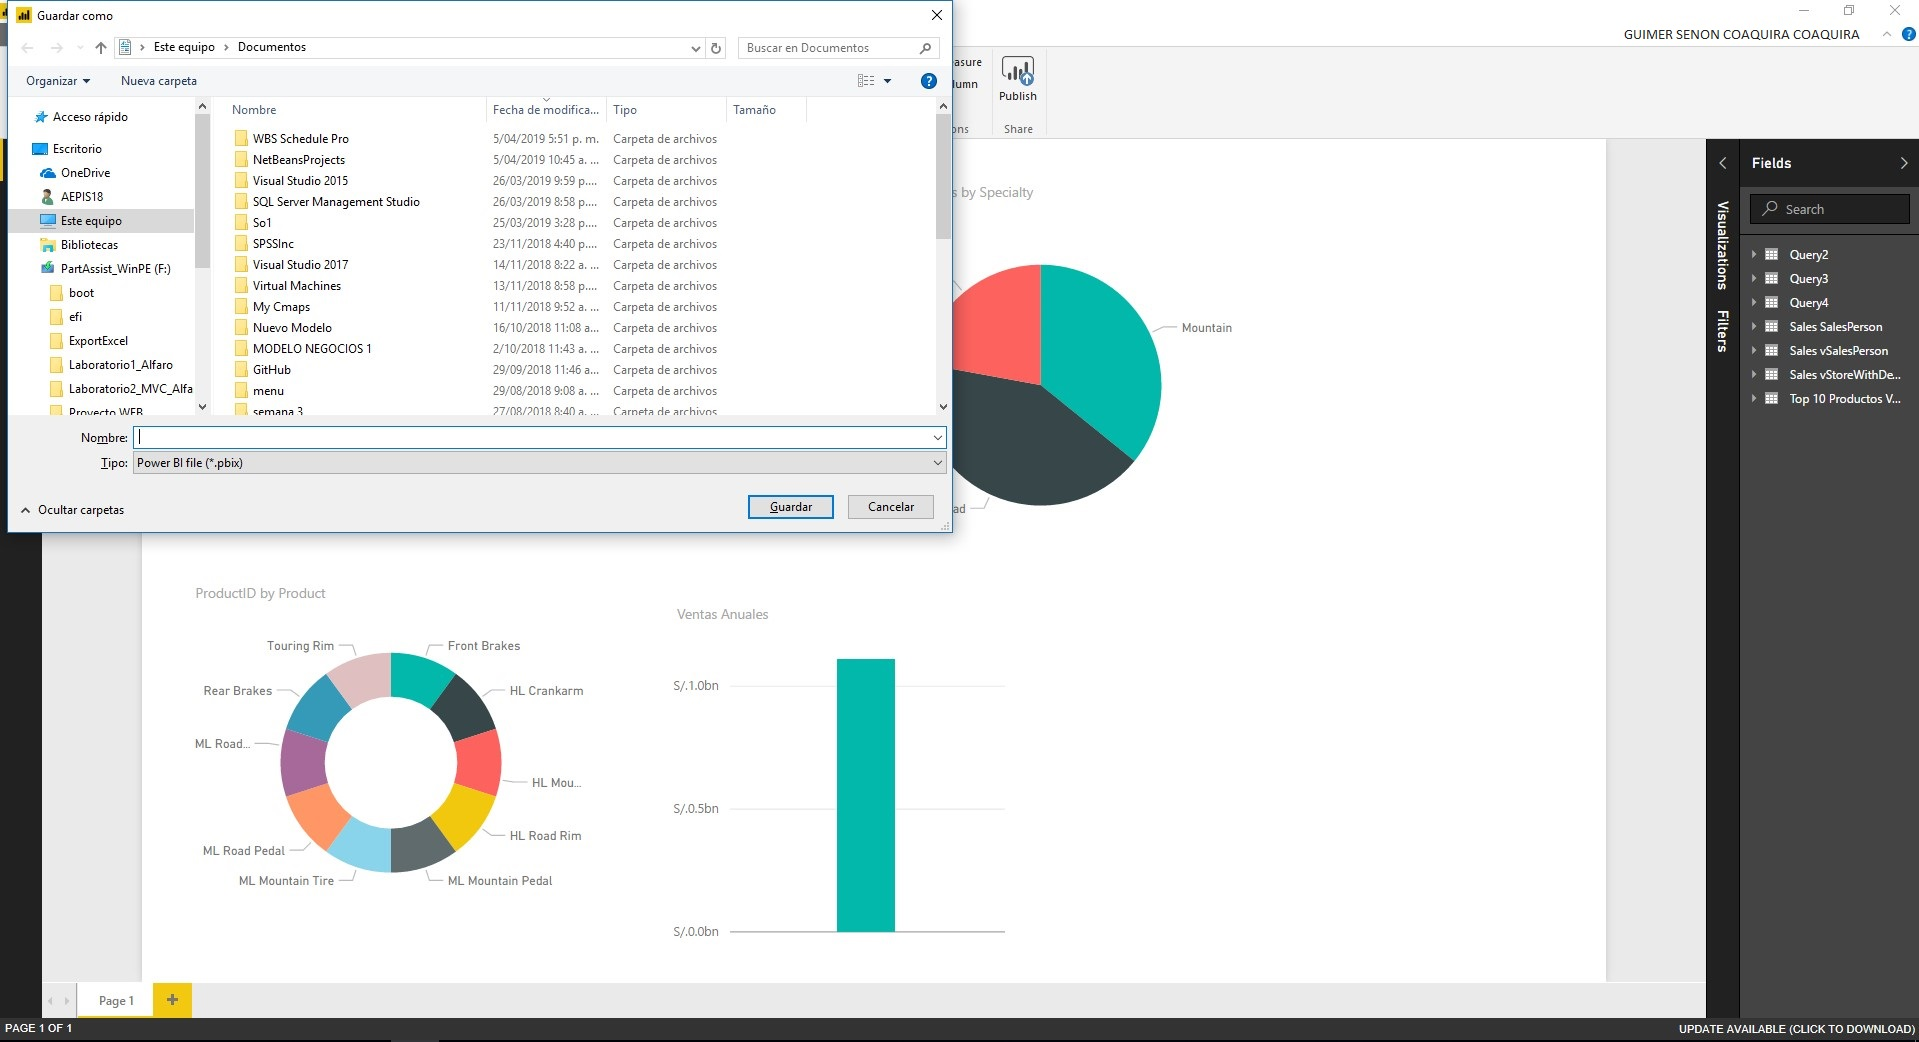
\includegraphics[width=15cm]{./Imagenes/Captura05}
\end{center}
\end{figure}

\subsection{RESULTADO Nº06:}
\begin{figure}[httb]
\begin{center}
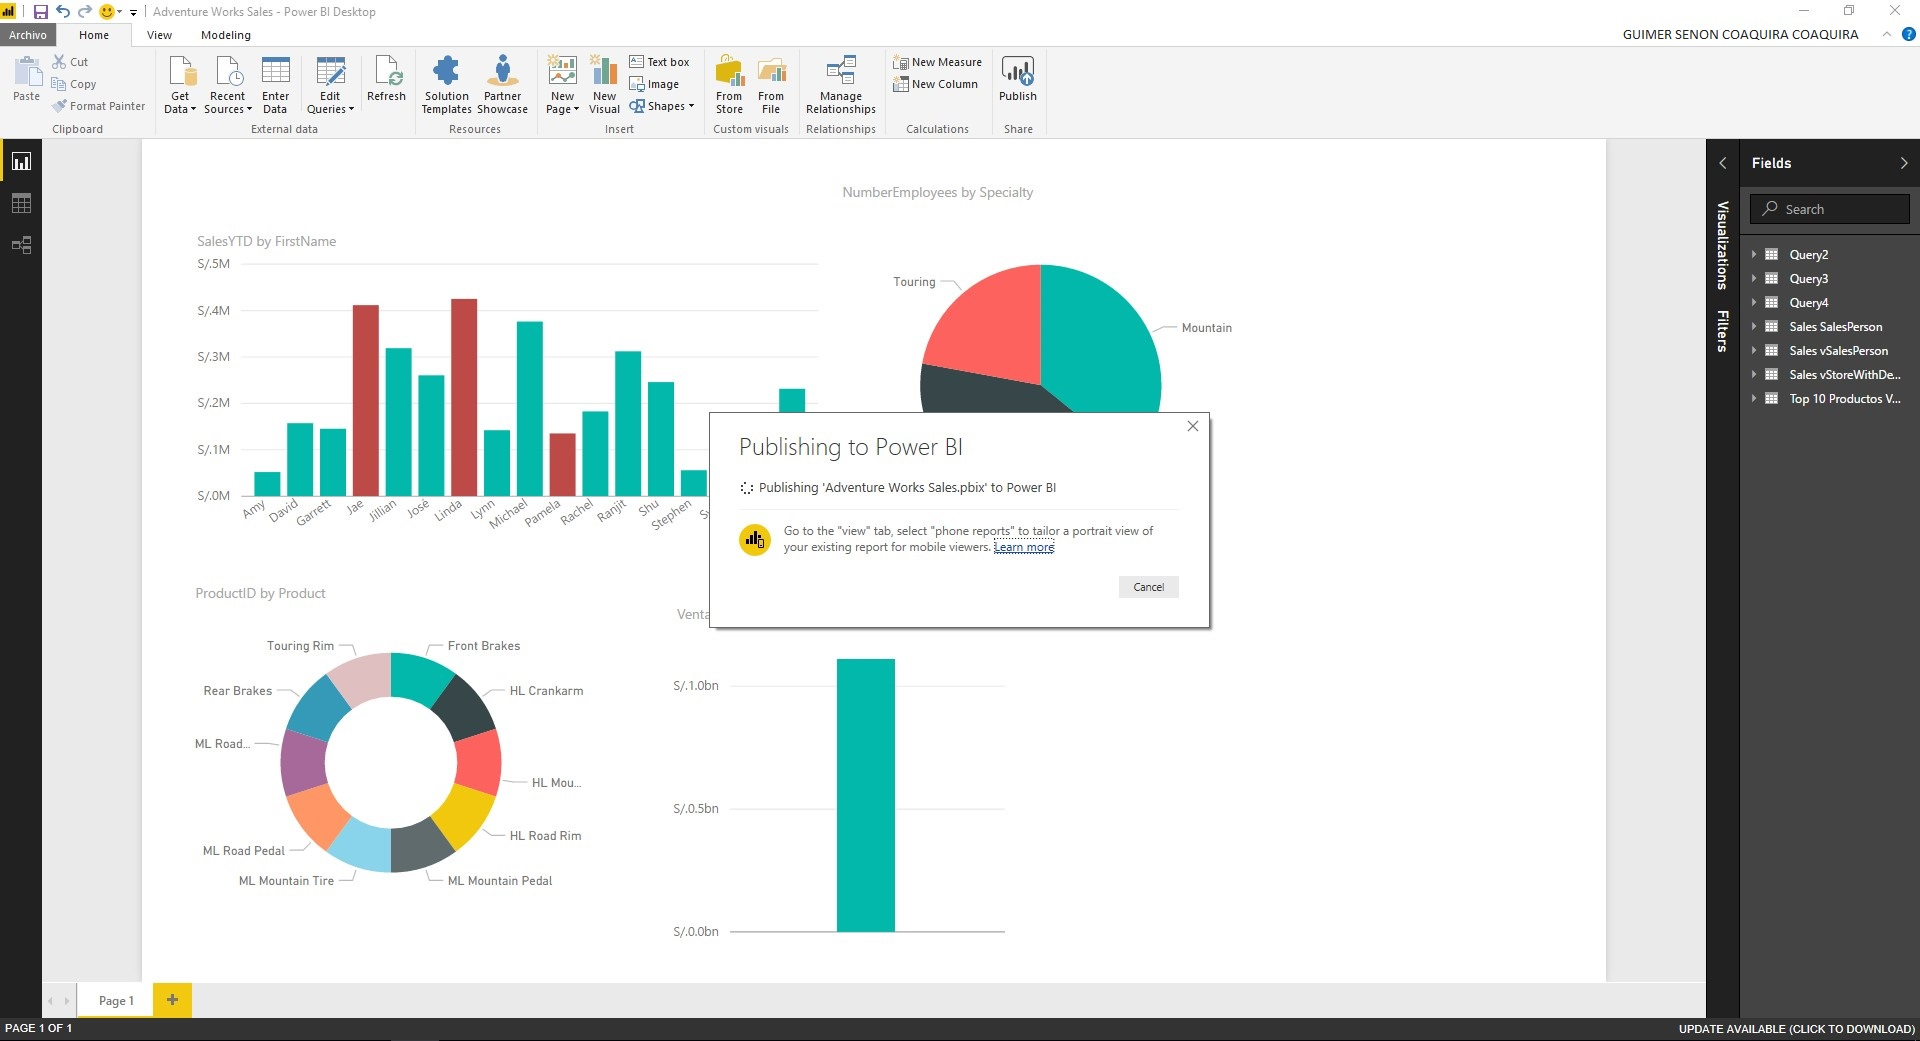
\includegraphics[width=15cm]{./Imagenes/Captura06}
\end{center}
\end{figure}